\documentclass{article}

\usepackage{Engineering}
\pdftitle{Electrical-eng}

% === TEXT ===
\title{\textbf{Electrical Engineering \\ HSLU, Semester 2}}
\author{Matteo Frongillo}
\date{}

\begin{document}

\maketitle
\tableofcontents
\pagebreak

\part{...}
\section{...}
\subsection{Current strength or current ``I''}
\begin{center}
    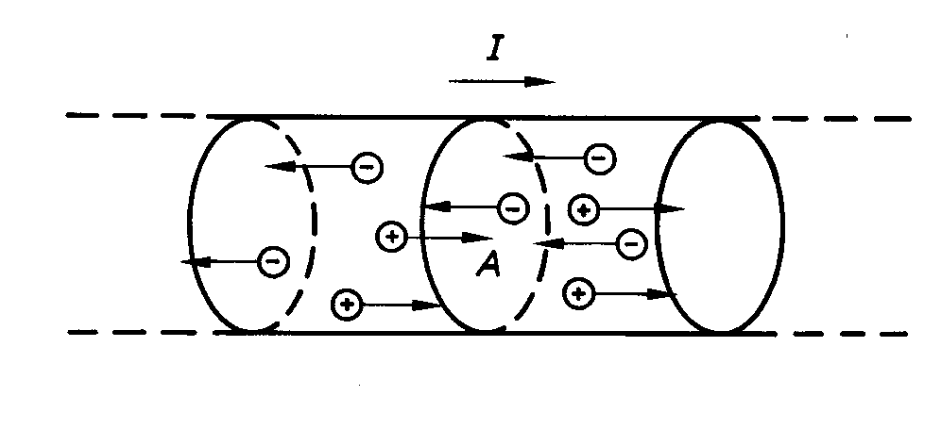
\includegraphics[width=.4\textwidth]{media/intensity.png}
\end{center}
\[I\ [A] =\dfrac{\text{el. charge}}{t}\]

\subsection{Current density ``J''}
\begin{center}
    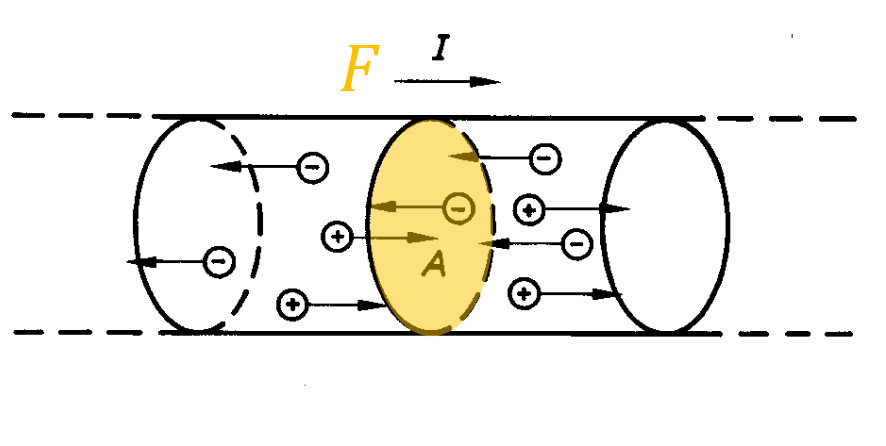
\includegraphics[width=.4\textwidth]{media/density.png}
\end{center}
The current density indicates how large the current per cross-sectional area (F) is:
\[J\ [\dfrac{A}{mm^2}] = \dfrac{I}{F}\]

\subsection{Temperature dependence of the resistance}
\begin{center}
    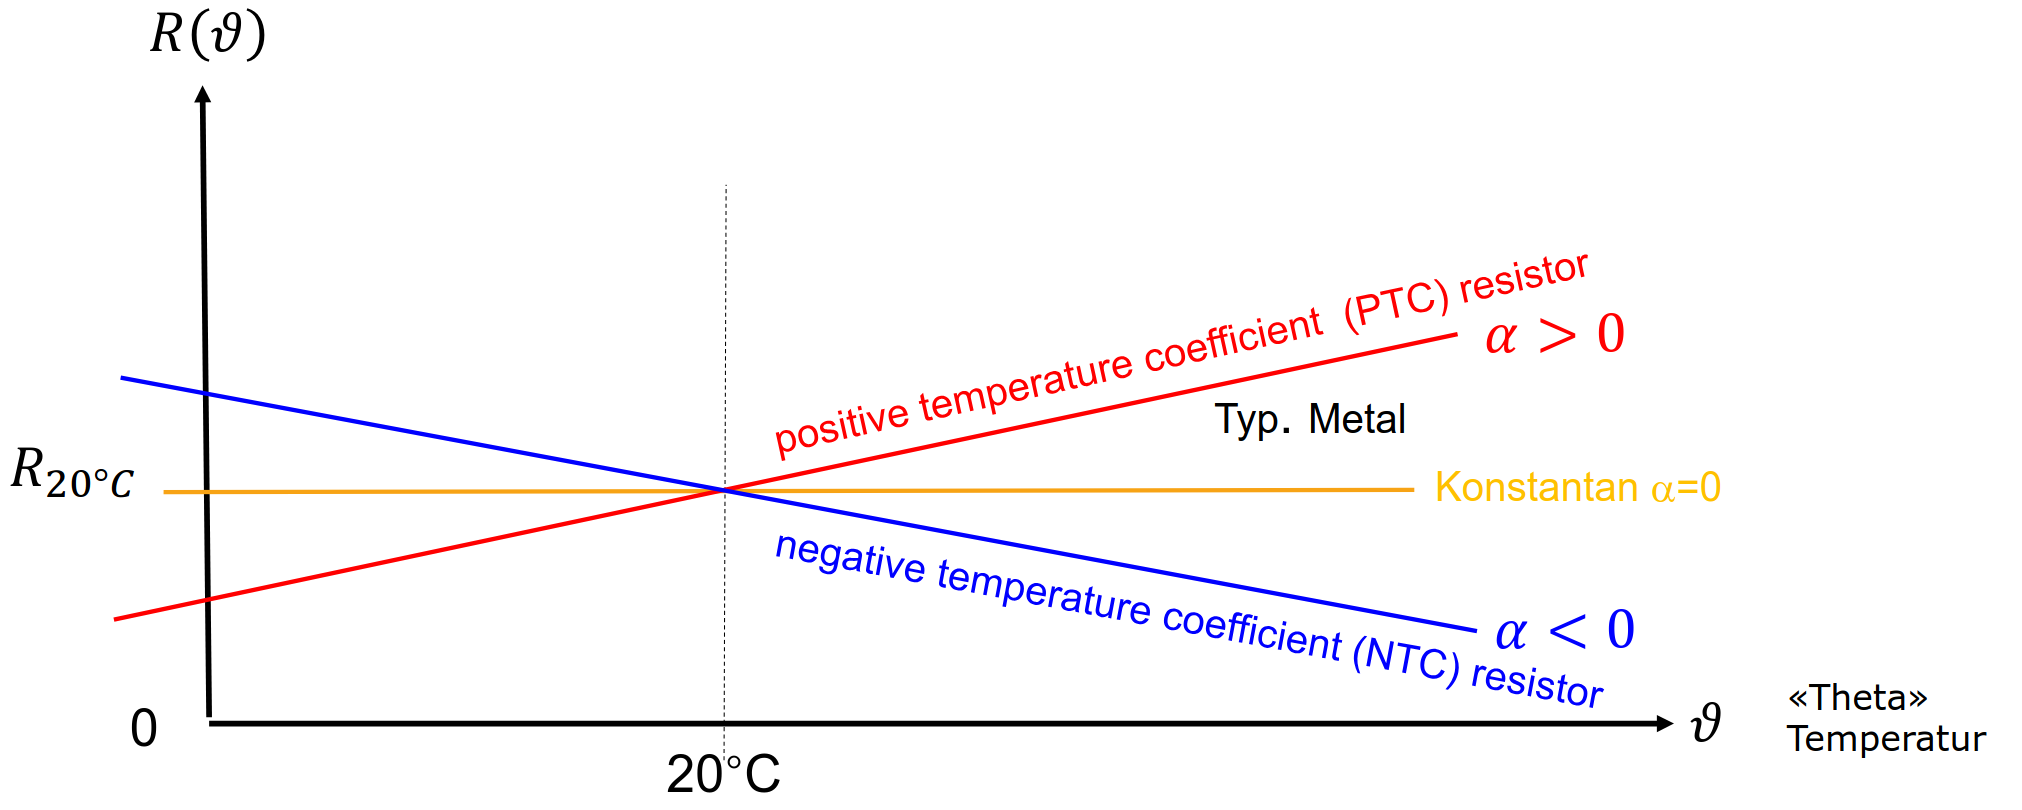
\includegraphics[width=\textwidth]{media/resistance.png}
\end{center}
Depending on the material, the resistance can increase, remain the same or decrease with temperature. In
ET+L we calculate using the linear approach.
\figbox{$R(\vartheta) = R_{20}(1+\alpha(\vartheta-20^{\circ}\text{C})) = R_{20}(1+\alpha \Delta T)$}

\subsection{Object properties}
The resistance indicates the voltage required for a
current. In addition to the material, the cross-sectional
area and also the length are decisive factors.
\[R=\frac{U}{I}\]

\subsection{Reciprocal quantities}
\subsubsection{Specific resistance}
To describe material properties, the resistance per length
and cross-sectional area is specified (precondition:
homogeneous conductor, direct current):
\[\rho\ [\frac{\Omega \cdot mm^2}{m}] = R\cdot \frac{A}{l}\]

\subsubsection{Conductance}


\subsubsection{Specific conductivity}

\newpage
\section{Gravitational fields}
\subsection{Between bodies}
\efigbox{F_1 = F_2 = G\dfrac{m_1m_2}{d^2}}

\subsection{Between particles}
\subsubsection{Coulomb's law}
It calculates the amount of force between two electrically charged
particles at rest:
\efigbox{F=\dfrac{1}{4\pi \varepsilon_0} \cdot \dfrac{q_1q_2}{r^2}}

where:
\begin{itemize}
    \item $F$: Force [N];
    \item $q$: Charge [As];
    \item $\varepsilon_0$: absolute permittivity = $8.8542\cdot 10^{-12}$ [As/Vm].
\end{itemize}

\subsection{Electric field and force on a charge $Q$}
\subsubsection{Homogeneous electric fields}
\efigbox{E=\dfrac{U}{d}}

where:
\begin{itemize}
    \item $E$: electric field strength [V/m];
    \item $U$: voltage [V];
    \item $d$: distance of the electrodes [m].
\end{itemize}

\subsubsection{Force on a point charge}
\efigbox{F=Q\cdot E}

where:
\begin{itemize}
    \item $E$: electric field strength [V/m];
    \item $Q$: charge [As];
    \item $F$: force [N].
\end{itemize}

\newpage
\section{Capacitance and Capacitor}
\subsection{Capacitor}
A capacitor is a device in which the capacitance is used.

\subsection{Capacitance}
Capacitance $C$ is the \textbf{capability} to store electric charge.
It is measured by the charge divided by the applied voltage:
\efigbox{C=\dfrac{Q}{U}}

where:
\begin{itemize}
    \item $Q$: charge [As];
    \item $U$: voltage [V];
    \item $C$: capacitance [As/V = F (Farad)].
\end{itemize}

\subsubsection{Capacitance of a plate capacitor}
\efigbox{C=\varepsilon\cdot \dfrac{A}{d}}

where:
\begin{itemize}
    \item $A$: plate area (one side) [m$^2$];
    \item $d$: distance between plates [m];
    \item $C$: capacitance [F].
\end{itemize}

\pph{Permittivity}
\efigbox{\varepsilon = \varepsilon_r\cdot \varepsilon_0}
\begin{itemize}
    \item $\varepsilon_r$: relative permittivity of the dielectric, relative to the air;
    \item $\varepsilon_0$: absolute permittivity [As/Vm].
\end{itemize}

\subsubsection{Energy in a capacitor}
If a capacitor is discharged with a constant current, the voltage decreases linearly:

\efigbox{\int_{0}^{t_{\text{empty}}}U(t)\cdot I\,dt = I\cdot U_0 = \frac{I\cdot U_0 \cdot t_{\text{empty}}}{2}}

Or, simplified:
\efigbox{W=\frac{1}{2}C\cdot U_0^2}

where:
\begin{itemize}
    \item $W$: energy [J or Ws];
    \item $U_0$: initial voltage [V];
    \item $C$: capacitance [F].
\end{itemize}

\subsection{Capacitors in parallel connection}
Capacitances connected in parallel add up:
\efigbox{C_{\text{tot}} = \frac{\sum_{n} Q_n}{U} = \sum_{n} C_n}

or

\efigbox{C = \frac{\varepsilon\cdot \left(\sum_{n} A_n\right)}{d} = \sum_{n} C_n}

\subsection{Capacitors in series connection}
In a series connection, the reciprocal of the total capacitance is the sum of the reciprocals of the individual capacitances:
\efigbox{\frac{1}{C_{\text{tot}}} = \sum_{n}\frac{1}{C_n}}

where:
\begin{itemize}
    \item $C_{\text{tot}}$: total capacitance [F];
    \item $C_n$: capacitance of the $n$-th capacitor [F].
\end{itemize}

\section{Transient Analysis in RC Circuits}
\subsection{Charging of a Capacitor}
When a capacitor is charged through a resistor, the voltage across it increases exponentially:
\efigbox{U_C(t)= U_0\cdot\left(1-e^{-t/(R\cdot C)}\right)}

with the time constant defined as:
\efigbox{\tau=R\cdot C}

where:
\begin{itemize}
    \item $U_C(t)$: voltage across the capacitor at time $t$ [V];
    \item $U_0$: applied voltage [V];
    \item $R$: resistance [$\Omega$];
    \item $C$: capacitance [F];
    \item $\tau$: time constant [s].
\end{itemize}

\subsection{Discharging of a Capacitor}
When a charged capacitor discharges through a resistor, the voltage decays exponentially:
\efigbox{U_C(t)= U_0\cdot e^{-t/(R\cdot C)}}

and the discharging current is:
\efigbox{I(t)= \frac{U_0}{R}\cdot e^{-t/(R\cdot C)}}

\newpage
\subsection{Transitional phase}
\efigbox{f(t)=A+\Delta\cdot \left(1-e^{t/\tau}\right) = A+(B-A)\cdot (1-e^{1/\tau})}

\section{Additional Topics}
\subsection{Energy Stored in a Capacitor}
The energy stored in a capacitor is given by:
\efigbox{W=\frac{1}{2}C\cdot U_0^2}

where:
\begin{itemize}
    \item $W$: energy [J];
    \item $C$: capacitance [F];
    \item $U_0$: voltage [V].
\end{itemize}

\subsection{Charge--Voltage Relationship}
For an ideal capacitor, the relationship between charge and voltage is:
\efigbox{Q=C\cdot U}

Moreover, the current is the time derivative of the charge:
\efigbox{I=\frac{dQ}{dt}=C\cdot\frac{dU}{dt}}

Note that the voltage across an ideal capacitor cannot change instantaneously.

\newpage
\section{Electromagnetic fields}
\subsection{Hans Christian Ørsted Observation}
\begin{center}
    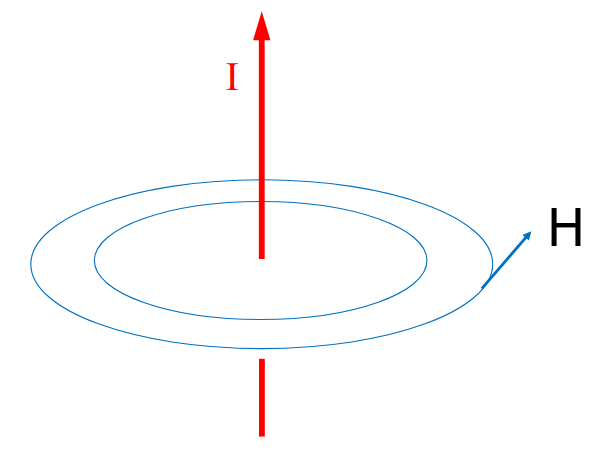
\includegraphics[width=.4\textwidth]{media/observations.png}
\end{center}
\begin{enumerate}
    \item The magnetic field lines encircle the current-carrying conductor;
    \item The magnetic field lines lie in a plane perpendicular to the current-carrying wire;
    \item If the direction of the current is reversed, the direction of the magnetic field lines is also reversed;
    \item The strength of the field is directly proportional to the magnitude of the current;
    \item The strength of the field at any point is inversely proportional to the distance of the point from the wire.
\end{enumerate}

\subsection{Definitions and formuals}
\subsubsection{Magnetomotive force}
\efigbox{\theta = N\cdot I}

\subsubsection{Ampère's circuital law}
\efigbox{\theta = \oint \overrightarrow{H(s)}\cdot \mathrm{d}\vec{s}}

\subsubsection{Magnetic field in a coil}
\begin{center}
    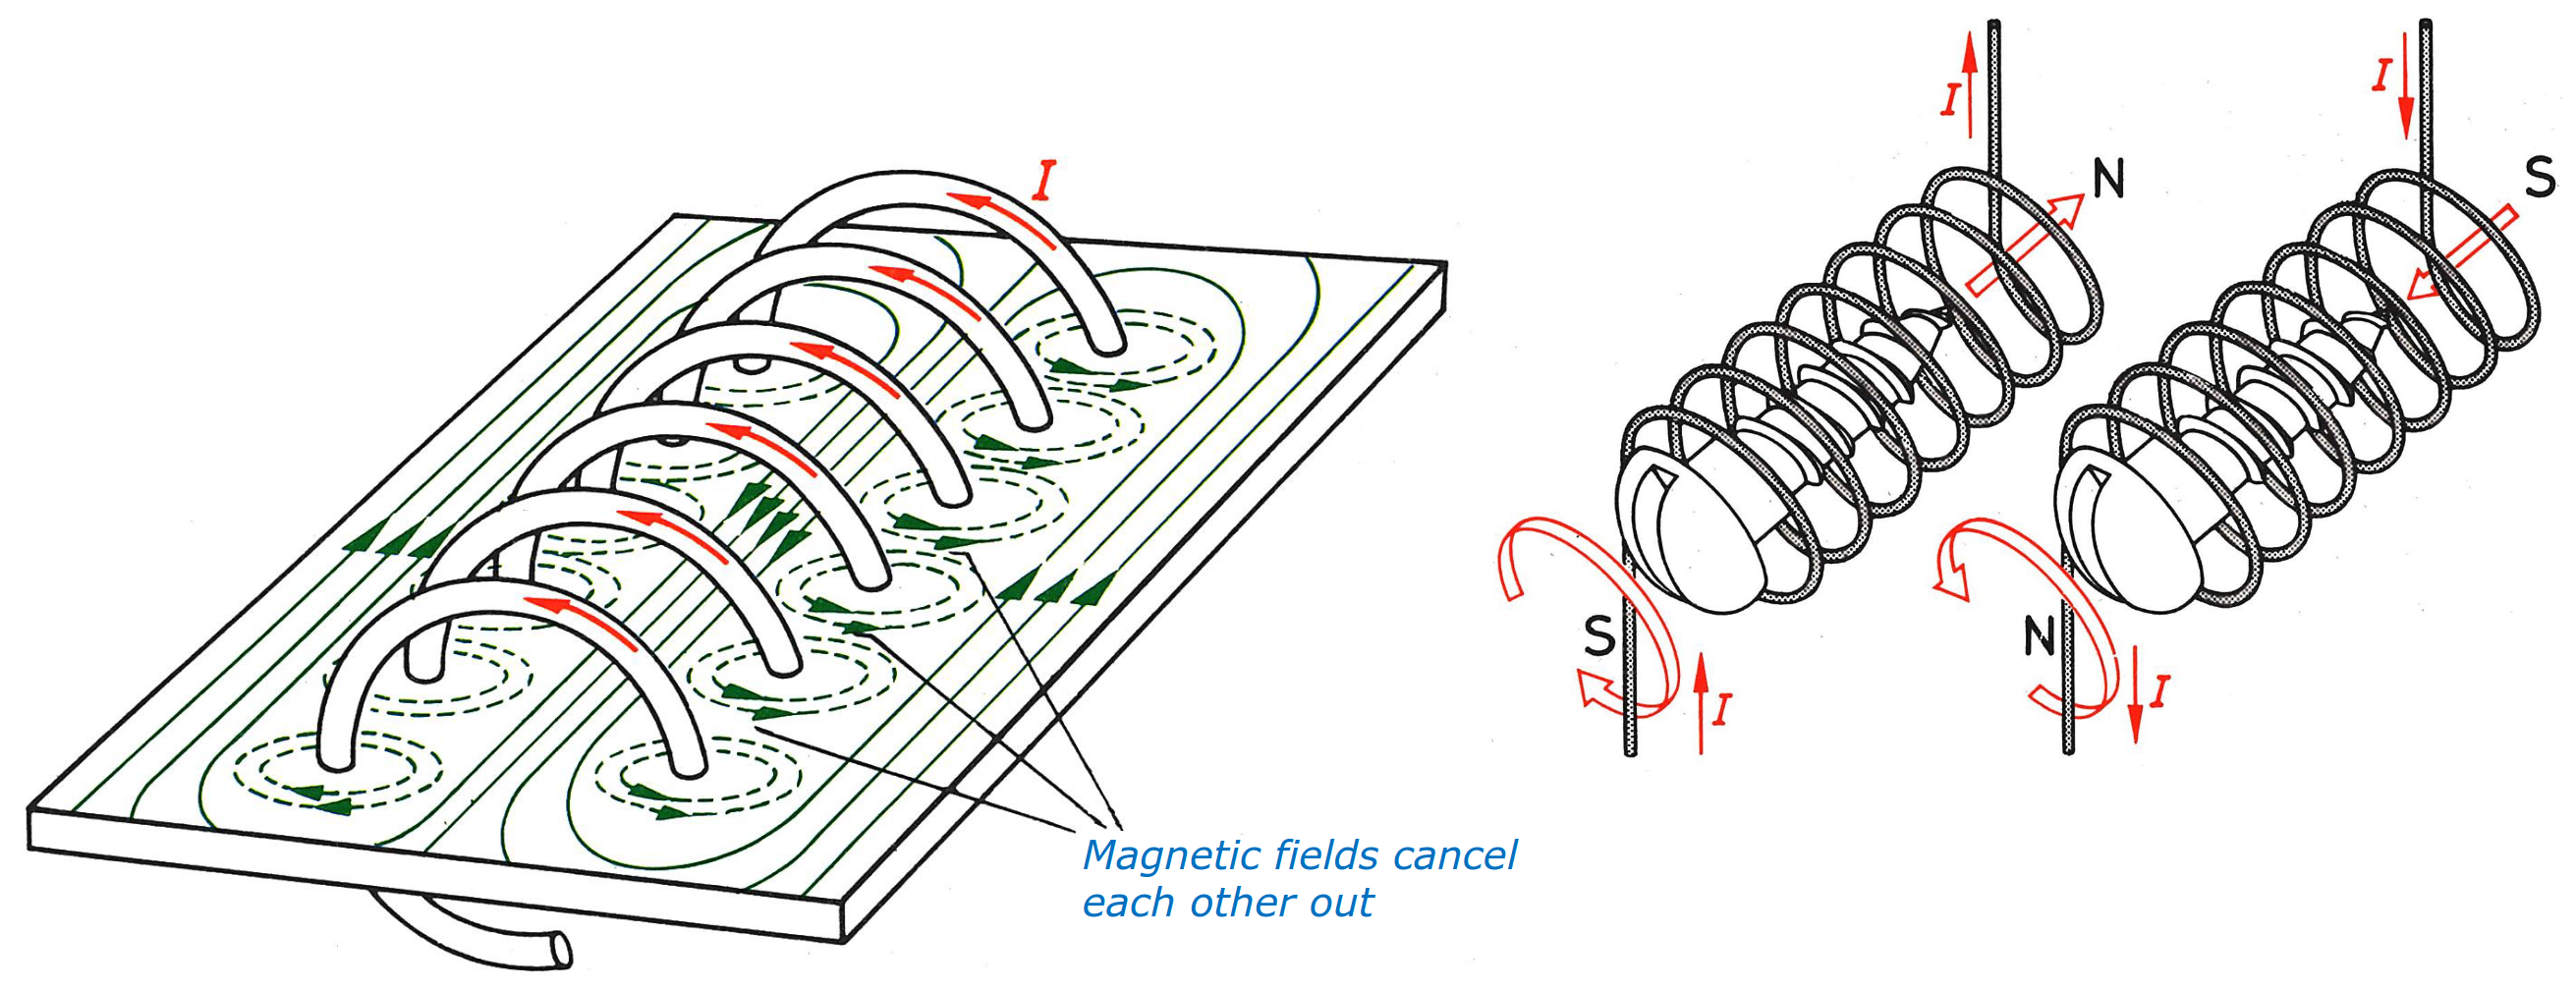
\includegraphics[width=\textwidth]{media/magneticfield_coil.png}
\end{center}

\newpage
\subsubsection{Magnetic flux density}
\efigbox{B = \frac{\Phi}{A} = \mu \cdot H = \mu_0\mu_r\cdot H}

where:
\begin{itemize}
    \item $B$: magnetic flux density [T = Vs/m$^2$];
    \item $\Phi$: magnetic flux [Wb];
    \item $A$: area [m$^2$];
    \item $\mu$: magnetic permeability [H/m = Vs/Am];
    \item $H$: magnetic field strength [A/m];
    \item $\mu_0$: magnetic constant [$4\pi\cdot 10^{-7}$ Vs/Am];
    \item $\mu_r$: relative permeability.
\end{itemize}

\note{$\Phi$ is the sum of all B-field lines through the cross section A}

\subsubsection{Magnetic field strength in coil with iron core}

\begin{center}
    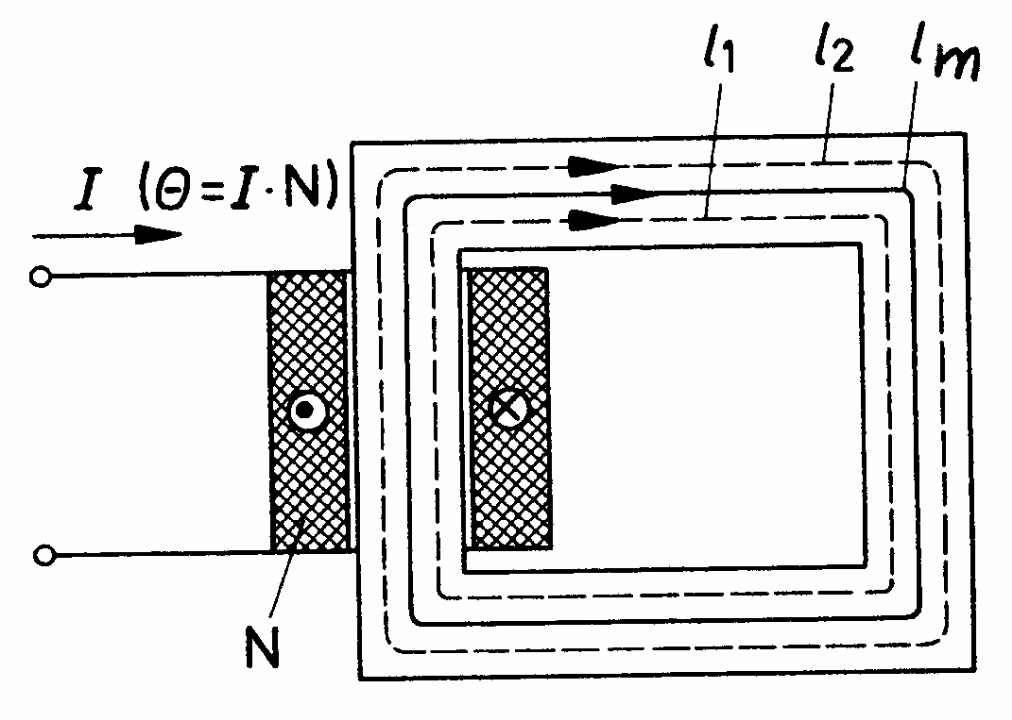
\includegraphics[width=.4\textwidth]{media/strength_iron_core.png}
\end{center}

\efigbox{H = \frac{N\cdot I}{l_{m}} = \frac{\Theta}{l_{m}}}

where:
\begin{itemize}
    \item $H$: magnetic field strength [A/m];
    \item $N$: number of turns;
    \item $I$: current [A];
    \item $l_{m}$: median field line length [m];
    \item $\Theta$: magnetomotive force [A].
\end{itemize}

\subsubsection{Magnetic relative permeability $\mu$}
Permeability is a measure for the ability to conduct magnetic field lines:

\begin{center}
    \begin{tabular}{|l|l|}
        \hline
        \textbf{Material} & $\mathbf{\mu_r}$ \\
        \hline
        Air & 1 \\
        Pure iron & up to 250'000 \\
        Electrical steel & 500 \ldots 7000 \\
        Steel & 40 \ldots 7000 \\
        Water & 0.99991 \\
        \hline
    \end{tabular}
\end{center}

\newpage
\subsubsection{Coils with and without iron core}
The magnetization curve of a coil without a core
is linear, but there is significantly less flux
density B than with an iron core.
\begin{center}
    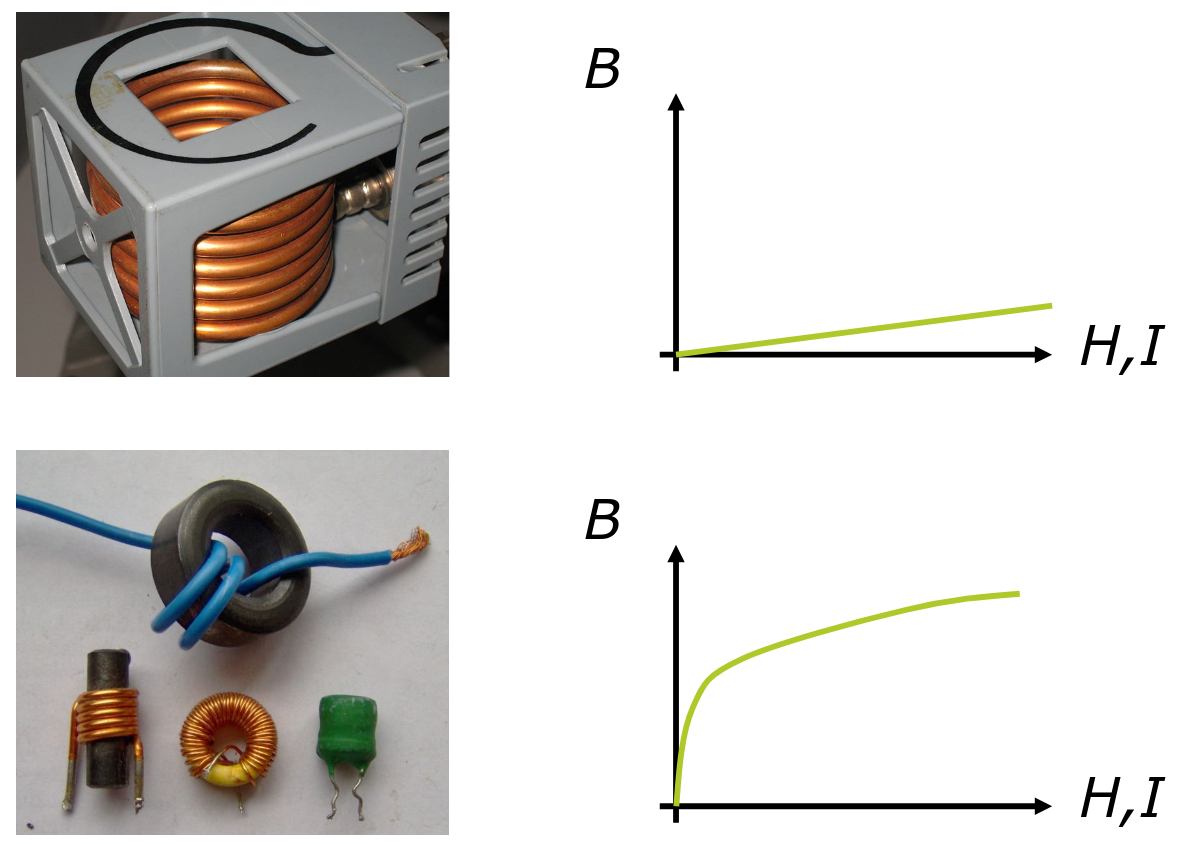
\includegraphics[width=.7\textwidth]{media/iron_coils.png}
\end{center}

\subsubsection{Law of induction and inductance}
\pph{Changing magnetic flux generates a voltage}
\begin{center}
    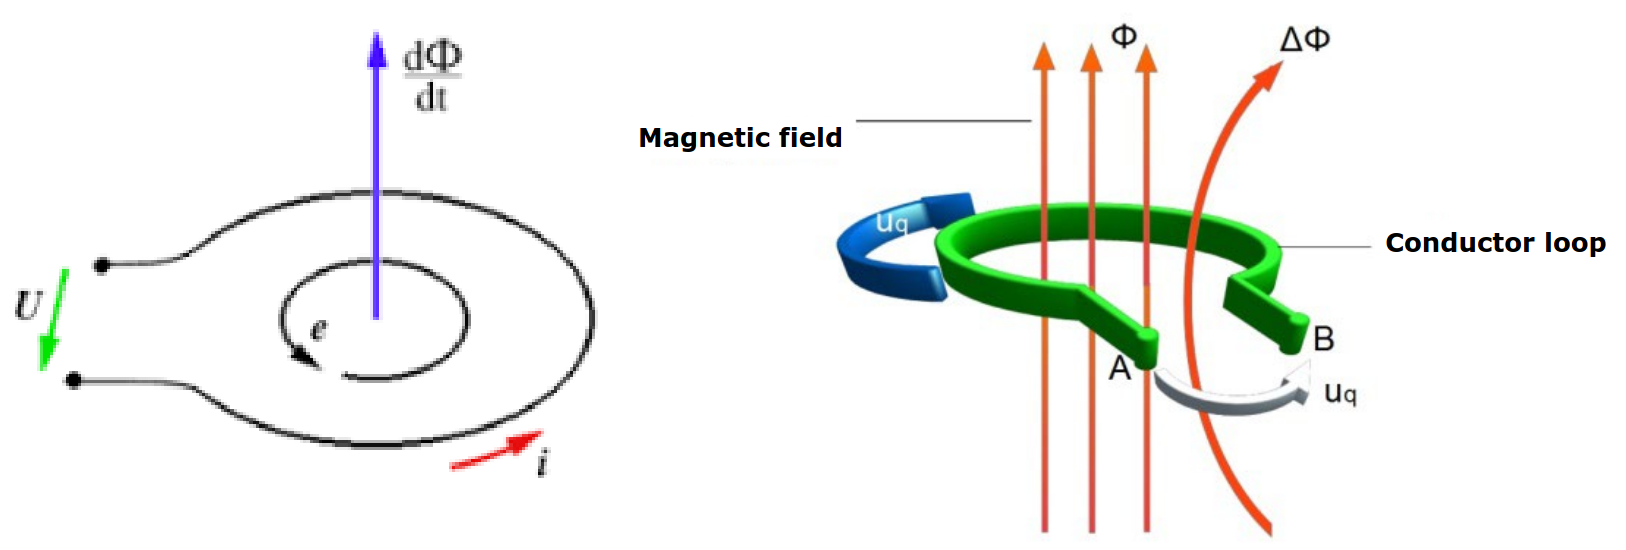
\includegraphics[width=.8\textwidth]{media/law_of_induction.png}
\end{center}

Phenomenon: a changing magnetic flux $\Phi$ induces a
voltage in a conductor loop around it:
\efigbox{U = -N\cdot \frac{\mathrm{d}\Phi}{\mathrm{d}t}}

\newpage
\subsubsection{Inductance and induction}
Inductance L is the capability to generate a magnetic field. It is measured by
the voltage divided by the rate of change of current over time. It is a measure of
the magnetic ``capacity'' of an arrangement of conductors (e.g. coil) and can be
compared to the capacity C of a capacitor. It indicates how much magnetic flux
per ampere is generated.

\efigbox{L = \frac{N\cdot \Phi}{I} = \frac{U}{\frac{\Delta I}{\Delta t}}}

where:
\begin{itemize}
    \item $L$: inductance [H = Vs/A];
    \item $N$: number of turns;
    \item $\Phi$: magnetic flux [Wb];
    \item $I$: current [A];
    \item $U$: voltage [V].
\end{itemize}

\subsubsection{Inductivity of a very long coil}
The inductance of a very long coil can be calculated approximately with:
\efigbox{L = \frac{\mu\cdot N^2\cdot A}{l}}

where:
\begin{itemize}
    \item $L$: inductance [H = Vs/A];
    \item $\mu$: magnetic permeability [Vs/Am];
    \item $N$: number of turns;
    \item $A$: cross-section of the coil [m$^2$];
    \item $l$: length [m].
\end{itemize}

\subsubsection{Energy stored in an inductor}
Since a variable magnetic field induces a voltage in which a current can also flow, the magnetic field must contain
energy:

\efigbox{W = \frac{1}{2}L\cdot I^2}

where:
\begin{itemize}
    \item $W$: work, energy [J = Ws];
    \item $L$: inductance [H = Vs/A];
    \item $I$: current [A].
\end{itemize}

\newpage
\subsubsection{Current-voltage relationship of an inductor}
The current-voltage relationship of an inductor is:
\efigbox{U = L\cdot \frac{\mathrm{d}I}{\mathrm{d}t}}

Special case:
\efigbox{0 = L\cdot \frac{\mathrm{d}I}{\mathrm{d}t} \rightarrow u_c = 0}

\subsubsection{Transient analysis}
\begin{center}
    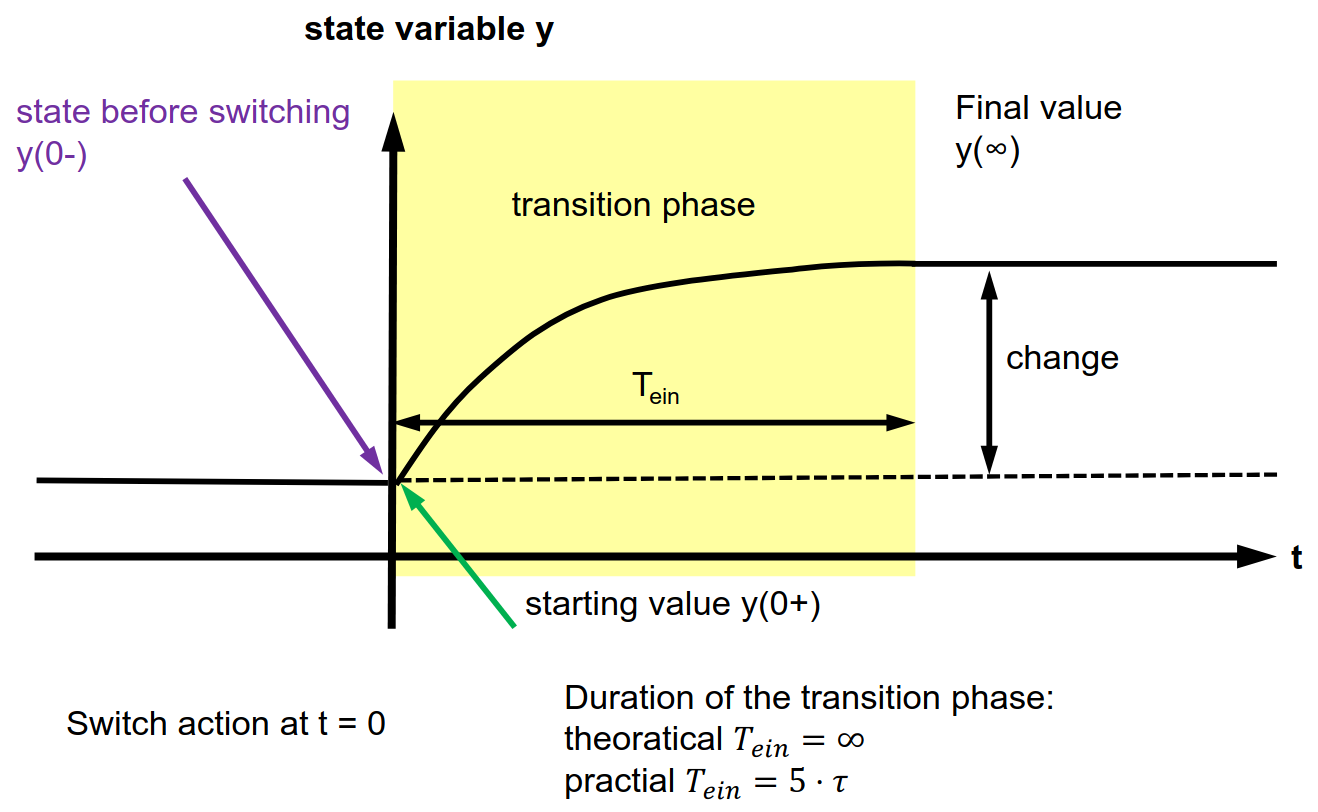
\includegraphics[width=.8\textwidth]{media/transient_analysis.png}
\end{center}

\begin{enumerate}
    \item The state variable $ y(t) $ is the variable that cannot change instantaneously.
    For the inductor, this is $ i_L(t) $. The state just before the switch action:
    \[
      y(0^-) = i_L(0^-).
    \]
  
    \item The starting value is the state immediately before the switch action:
    \[
      y(0^+) = i_L(0) = i_L(0^-).
    \]
    That is, the state variable $ i_L $ keeps the value from $ t = 0^- $.
  
    \item The final value is the value long after the switch action:
    \[
      y(\infty) = i_L(\infty),
    \]
    which is practically reached after $ 5\tau $.
  
    \item The transient is described by the function of time:
    \[
      y(t) = \text{final value}
      + \bigl(\text{starting value} - \text{final value}\bigr)\, \exp{\left(-\frac{t}{\tau}\right)}.
    \]
    Hence,
    \[
      i_L(t) = i_L(\infty)
      + \Bigl(i_L(0+) - i_L(\infty)\Bigr)\, \exp{\left(-\frac{t}{\tau}\right)}.
    \]
\end{enumerate}

\newpage
\pph{Time constant $\tau$ for an inductor}
\efigbox{\tau = \frac{L}{R}}

where:
\begin{itemize}
    \item $\tau$: time constant [s];
    \item $L$: inductance [H];
    \item $R$: resistance [$\Omega$].
\end{itemize}

\subsection{Examples}
\subsubsection{Charging an inductor in a RL-network}
\begin{center}
    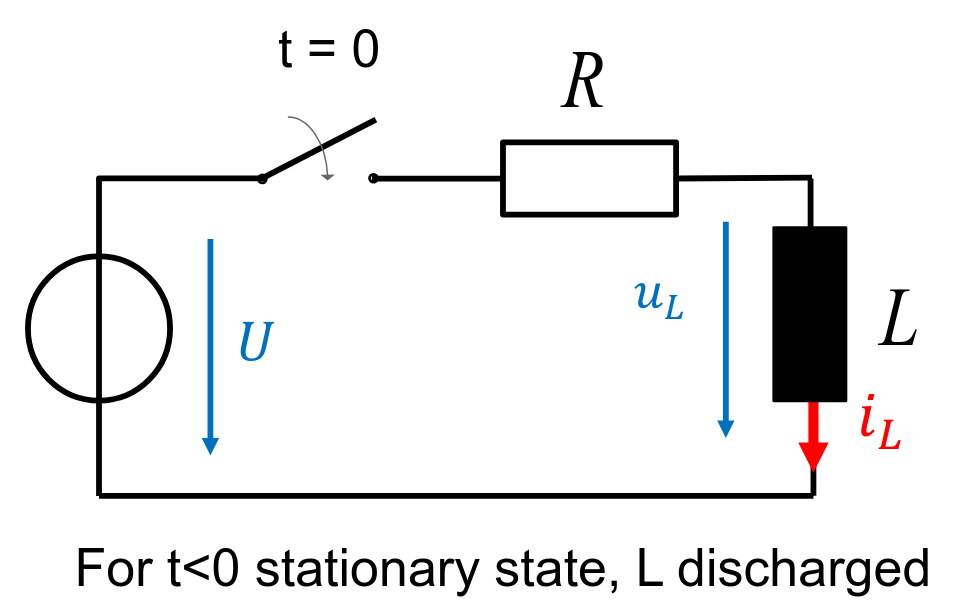
\includegraphics[width=.5\textwidth]{media/inductor_ex1.png}
\end{center}

\pph{Calculations}
\efigbox{i_L = \frac{U}{R}\cdot \left(1-\exp{\left(-\frac{t}{\tau}\right)}\right)\\\\\\
        u_L = U\cdot \exp{\left(-\frac{t}{\tau}\right)}}

\pph{Graphical representation}
\begin{center}
    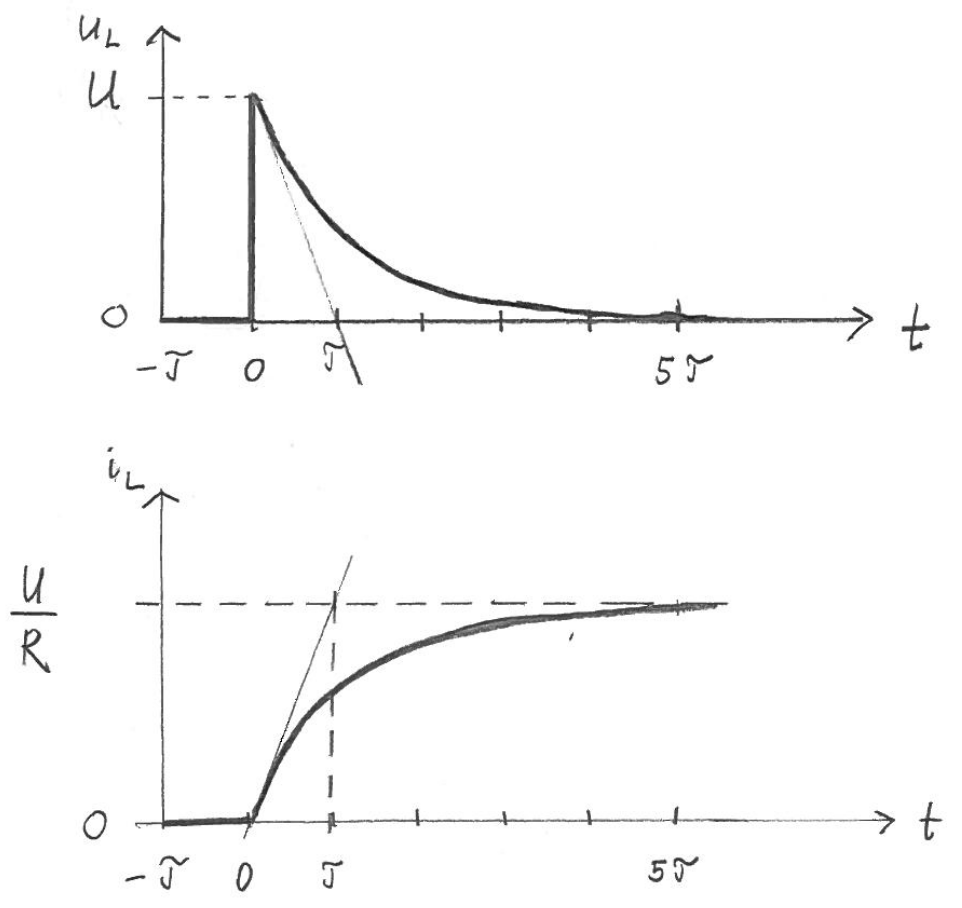
\includegraphics[width=.45\textwidth]{media/inductor_ex1_graph.png}
\end{center}

\newpage
\subsubsection{Discharging an inductor in a RL-network}
\begin{center}
    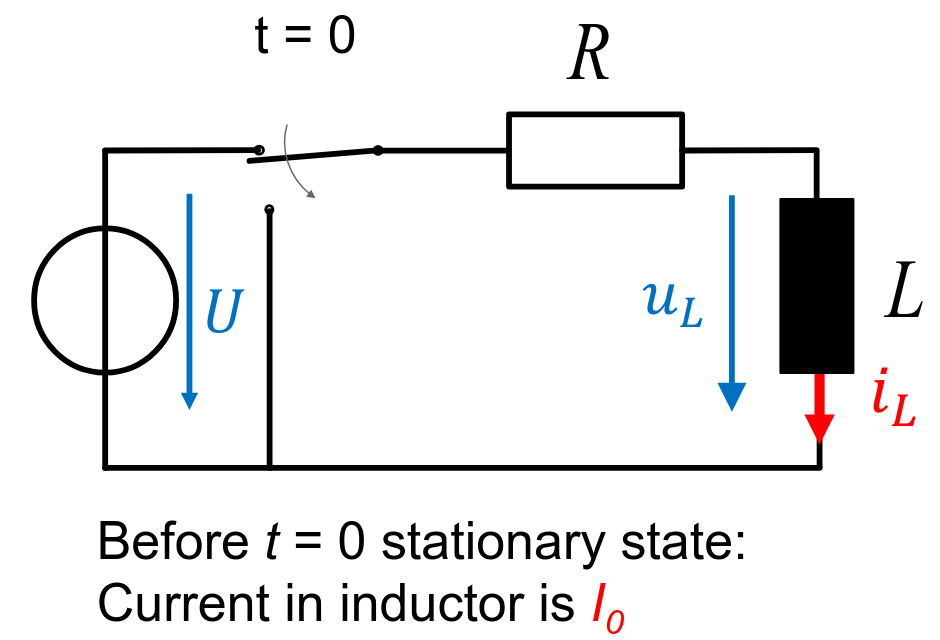
\includegraphics[width=.5\textwidth]{media/inductor_ex2.png}
\end{center}

\pph{Calculations}
\efigbox{i_L = I_0\cdot \exp{\left(-\frac{t}{\tau}\right)}\\\\\\
        u_L = -I_0\cdot R\cdot \exp{\left(-\frac{t}{\tau}\right)}}

\pph{Graphical representation}
\begin{center}
    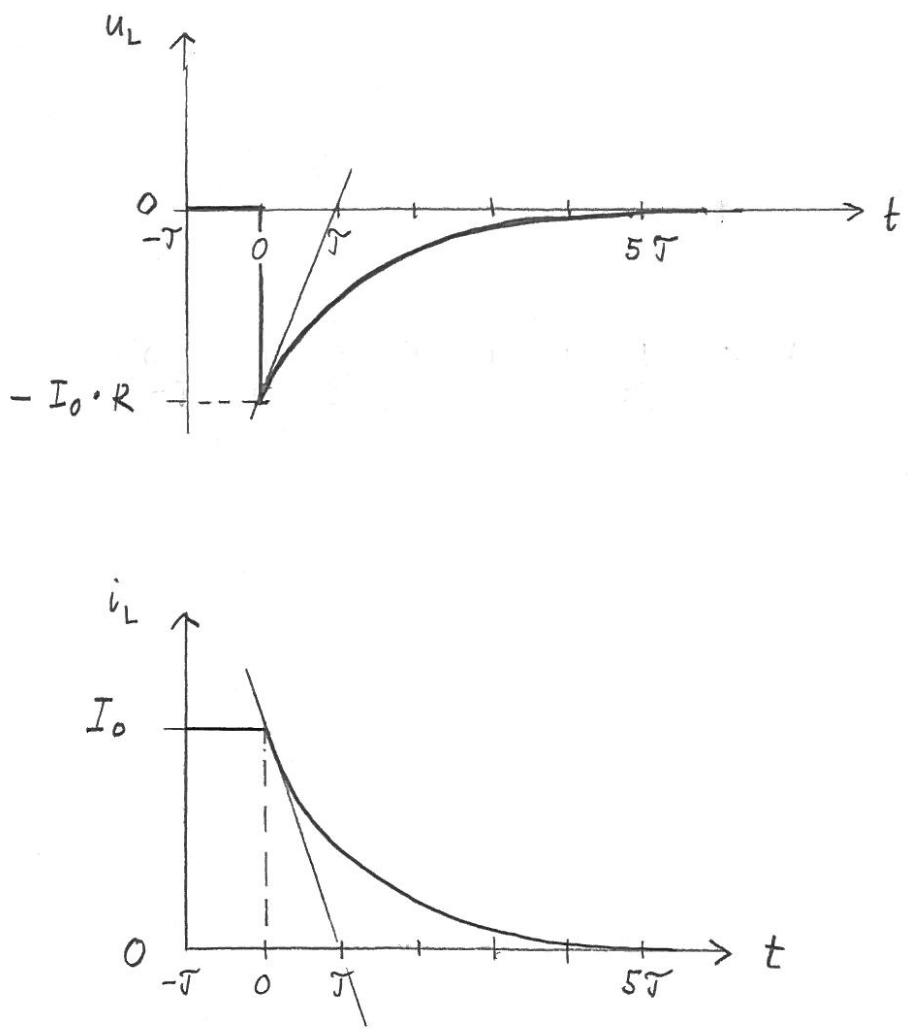
\includegraphics[width=.45\textwidth]{media/inductor_ex2_graph.png}
\end{center}







\end{document}
